\documentclass[12pt]{article}
\usepackage[utf8]{inputenc}
\usepackage{amsmath}
\usepackage[backend=biber]{biblatex}
\usepackage{graphicx}
\addbibresource{ref.bib}

\title{Can Numba and CUDA Python Development Kits be used on a GPU to Speed Up 2D Gamma Index Calculations used in Radiotherapy?}

\author{
  Sun, Edward$^{1}$
}
\date{%
  $^{1}$Torrey Pines High School, San Diego, California
  \today
}

\begin{document}

\maketitle
\section{Introduction}
\subsection{Radiotherapy Background}
Cancer is the second leading cause of death following heart disease. In 2020 alone, cancer alone was responsible for the deaths of 602,350 deaths in the United states (\textcite{CDC}). However, with the aid of modern radiotherapy procedures, this figure can be significantly reduced. Starting with the invention of the X-ray by the German scientist Conrad Roentgen, radiotherapy had made great strides in development more and more precise ways of targeting cancer cells and sparing health tissue. Begining with crude methods involving radium and low-voltage diagnostic X-ray machines, today radiotherapy has evolved into a complicated procedure that involves various imaging modes and treatment deliver modes that ensure the highest accuracy. This procedure of radiotherapy is defined to include: patient consultation, simulation, treatment planning, and treatment delivery (\textcite{SBU}). In the patient consultation step, patients are initially diagnosed and informed of their condition. Following the consultation, the patients are taken to imaging facilities to capture images of their tumor(s) where contrast agents/chemicals are used to exaggerate the location of the tumor(s). Computer simulations are then used to define the location of the tumor and configurations of the treatment. Following this is the treatment planning step, where radiation oncologists, physicists, and dosimeters are involved to plan the radiotherapy for the patient. The goal of this step is to deliver high doses to the tumor while limiting the damage to the surround health tissues, thereby reducing the side effects of radiotherapy.

\subsection{Quality Assurance}
As modern radiotherapy is a complex process that involve many steps as mentioned above, quality assurance (QA) methods are needed to reduce errors and ensure the quality of results before moving on to delivering the doses on the patients. One of the most important QA steps is the assurance of the delivered doses with the calculated doses of a treatment planning system. In planning the treatment based on a patient's body, a commercial treatment planning system is often used to calculate treatment plans or how much radiation to send to a specific location (\textcite{Gardner}). Due to the sensitivity of radiotherapy, these treatment planning system is often routinely requires the comparison of measured and calculated dose distributions (how the doses are delivered across a part of the patient's body). Given the tumor information of the patient, the treatment planning system will generate radiation delivery plans.


\begin{figure}[h]
  \centering
  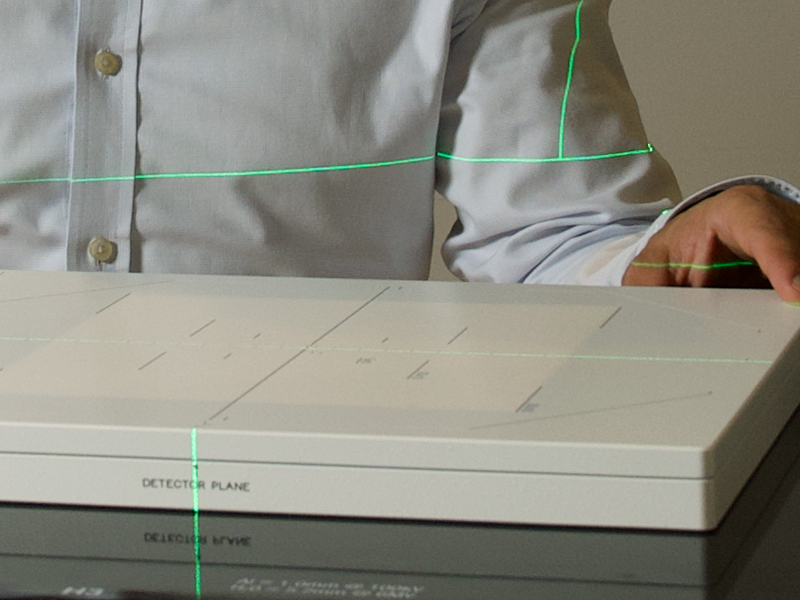
\includegraphics[scale=1.2]{images/map.png}
  \caption{Sun Nuclear MapCHECK3 Radiation QA Matrix}
  \label{fig:mat}
\end{figure}


However, to ensure the accuracy of dose delivery to the patient and minimize accidental radiation exposure, QA is essential to treatment planning. Techniques involved in this quality assurance steps often involve the comparison of dose distributions of a measured dose distribution, obtained from running the treatment plan on a radiation detection matrix (Figure \ref{fig:mat}) that is sensitive to radiation and will measure the specific doses delivered at specific coordinates (\textcite{sunnuclear}).


\begin{figure}[h]
  \centering
  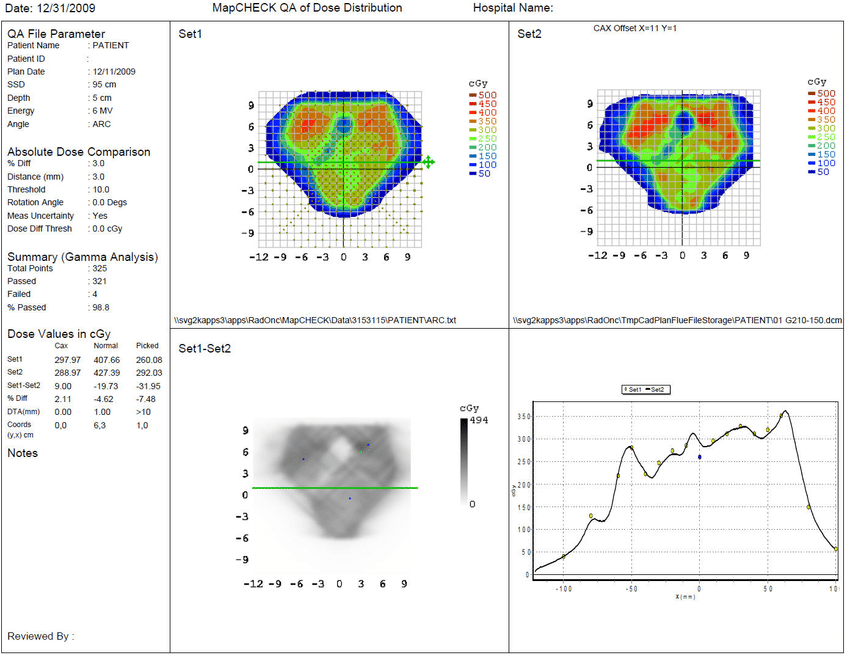
\includegraphics[width=\linewidth]{images/examplemap.png}
  \caption{Example MapCHECK QA (on left) and planned dose distribution (on right)}
  \label{fig:ex}
\end{figure}

An example of the measured dose distribution versus the planned can be seen in (This measured dose distribution will be compared against the intended/planned distribution with various mathematical comparison methods to judge the accuracy of the treatment planning system and make adjustments accordingly to ensure precision of treatment (\textcite{Low}).

\section{Literature Review}
\subsection{QA Methods}
Over the past decades, many metrics have been developed to improve QA. These methods are mathematical formulas/algorithms that often searches through and compares the calculated and measured dose distributions (dose images) in 2D or 3D to give a value that signifies the resemblance and therefore the accuracy of a treatment planner. For instance, Cheng $et. al$, used a pass-fail criteria for the dose difference (DD), which is the difference between the measured and calculated dose on a pixel, and distance to agreement (DTA), which is the distance/radius in which the algorithm searches on the dose distribution (\textcite{Cheng}). Each point within this search circle defined by the DTA is analyzed (Cheng). Similar metrics have been defined like the Global Gamma evaluation, maximum allowed dose difference (MADD) (Jiang), divide and conquer (D\&C) (\textcite{Stojadinovic}), and more. However, one metric has been defined as the standard of QA metrics in the field of radiotherapy, that is the gamma index (\textcite{Low}).

\subsection{$\gamma$ index}
The gamma index, originally proposed by Low et. al (\textcite{Low}), provides a representative and numerical metric that simultaneously incorporates the dose and distance criteria as mentioned above. It combines the ac curacies of previously proposed metrics into one $\gamma$ index. This formula is mathematically defined by the following formulas:
\\
\\
\begin{align}
  \Gamma = \frac{|dose_{planned} - dose_{actual}|}{dose_{threshold}} \\
\end{align}
\\
\\
This original formula for the simple gamma index is robust and reliable. The calculation is also relatively simple, as it is a simple subtraction, this calculation can be achieved with has been adopted and accepted widely. Since then, researchers have been making modifications to this algorithm adding more metrics for greater accuracy or changing the formula for greater efficency when running on computers' CPU or GPU (\textcite{Gu}).

One popular modification is to add DTA as a factor into the calculation of the index. Essentially, this modified algorithm is a iterative process which passes over every pixel on a dose distribution image. For the sake of easy understanding, we will use a 2D example, but the same logic can be applied for 3D dose distributions as well. To begin the search, we will start on one reference pixel (calculated dose distribution) and test pixel (measured dose distribution), where dose distributions in this case are defined as 2D grayscale images. Then, the iteration begins with defining a reference position in real units based on a pixel on the reference image and then iterating through the circle on the test image. Test pixel within this search radius is then evaluated with the formulas above along with a percentage passing criteria, which means that this pixel passes the $\gamma$ index test if it is within this many percentage relative to the reference pixel. During this process, as the iteration uses real units (mm), it may generate a position that does not land on a pixel. Here, interpolation is used to estimate the value at that position within the search radius. This search radius for each reference pixel is actually the DTA and the percentage is the DTA criterion.
>>>>>>> 4ad9b1ea5a9bf38c7509ee189a7fedf264133f3c
\\
\\
\begin{align}
  l = \sqrt{\frac{r^{2}(r_{m}, r)}{\Delta d^{2}_{M}} + \frac{\delta^{2}(r_{m}, r)}{\Delta D^{2}_{M}}} \\
  r(r_{m}, r) = \lvert r-r_{m} \lvert \\
  \delta(r_{m}, r) = D(r)-D_{m}(r_{m}) \\
  \gamma(r_{m}) = min\{\Gamma(r_{m}, r_{c})\forall(r_{c})\}
\end{align}
\\
\\
Mathmatically, as seen in the equations above, Eq. (1) describes the intermediate value $l$ calculated for each pixel, where $r^{2}(r_{m}, r)$ defines the square of the distance between the reference and the test pixel. The parameters $r_{m}$ of $r^{2}(r_{m}, r)$ is the real position of the measured pixel and r defines the real position of the test pixel, as pointed out by Eq. (2). $\delta^{2}(r_{m}, r)$ defines the square of the difference in pixel value (in real terms, pixel value is radiation dose intensity) where $r_{m}$ represents the pixel value of the measured pixel and $r$ represents the pixel value of the test pixel, as pointed out by Eq. (3). $r^{2}(r_{m}, r)$ is then divded by $\Delta d^{2}_{M}$ which is the DTA or search radius. $\delta^{2}(r_{m}, r)$ is then divded by $\Delta D^{2}_{M}$ which is the DTA criterion or acceptable passing percentage. This whole term is then square-rooted to produce the intermediate gamma value. This process is then repeated for all values within that radius for that refernce pixel. The final gamma index for that reference value is taken as the minimum value of all these previously calculated intermediate values. Then, this is repeated for all reference pixels from the reference image to produce one gamma value for each reference pixel, thereby creating a gamma image.

\subsection{Challenges to the $\gamma$ Index}
With such a iterative and complex system involving intensive interpolation and calulations, Gu et. al (\textcite{Gu}) highlighted the concerns of speed with the $\gamma$ index calculation, where clinically relevant dose distribution sizes is very time-consuming to compare. Many researchers have attempted to improve the accuracy and efficiency of the algorithm (\textcite{Bakai}, \textcite{Depuydt}, \textcite{Stock}, \textcite{Jiang}, \textcite{Spezi}) while others focused on speed (\textcite{Ju}, \textcite{Chen}, \textcite{Wendling}).

\subsection{Code Acceleration in Python}
Other than algorithmic approaches to speeding up the $\gamma$ index, another approach is to use a graphics processing unit (GPU) to accelerate time consuming code. GPUs are a part of a modern computer that accelerates the rendering of computer graphics, especially in games, content creation, etc. (\textcite{intel}). However, they have also been repurposed for scientific computing, which takes advantage of their high calculation powers. As seen, GPUs have been used in weather prediction (\textcite{Michalakes}), mechanical structural analysis (\textcite{Georgescu}), and chemical analysis (\textcite{Ma}). These studies typicall use Nvidia CUDA acceleration toolkits in the C programming language or they are built from the ground up.

However, within recent years, Python has been a popular choice within the area of GPU acceleration. This is largely thanks to the growing development in acceleration libraries like Numba (\textcite{Lam}). By itself, Numba is a Just-in-Time (JIT) compiler for Python, where code (in this case python code) is compiled into machine code during the execution of the python program rather than before the execution of the program. This compilation into machine code makes python code much faster as Python by itself, is interpreted during run time on a virtual machine and then executed. In recent years, Nvidia, the manufacturer of a majority of commerical graphics cards, have partnered with the developers of Numbda to create GPU support for Numba, which now not only enables Numba to do JIT compilation, but also use GPUs to accelerate code.

Implementation of the gamma index in python isn’t new. Many opensource repositories on github have produced efficient gamma index calculation scripts\footnote[1]{github.com/christopherpoole/pygamma} Similarly, Biggs et. al (\textcite{Biggs}) have proposed and maintained a community driven project named pymedphys where CPU driven gamma index codes and other medical physics related codes have been implemented. GPU acceleration with gamma index isn’t new either. For instance, Gu et. al had proposed gamma index acceleration with a GPU in 2005 (\textcite{Gu}). There have also been GPU acceleration toolkits released by MATLAB and researchers have implemented similar algorithms of the gamma index in MATLAB (\textcite{Matlab}). However, as seen, there is GPU acceleration in MATLAB, but not implemented with Numba and CUDA in python. Similarly, there have been gamma index implemented in python, however, there has not been GPU accelerated gamma index calculations.

Python is one of the most popular data analysis and processing tool in the software engineering world. With the popularity of this language, more tools should be made avaliable for use in research. Thus, the reasoning behind the choice of this project is due to the high popularity of python, the large community support for GPU acceleration in python, and the prevalent use of the gamma index in radiotherapy. This study aims to fill this gap by creating a GPU accelerated gamma index framework for 1D, 2D, and 3D dose distributions in python via Numba and python CUDA. This will be achieved with a Nvidia GTX 1080 GPU (\textcite{NVidia}) running on PopOS 22.05 LTS with Nvidia CUDA support built in. For the algorithm, this study will be based off of Low et. al (\textcite{Low})’s original gamma index paper witht no modifications made to the algorithm. This study aims to test the feasibility of implementing the gamma index with Numba and CUDA while also benchmarking this against other frameworks within other languages (MATLAB, C, etc) to analyze if Python Numba and CUDA accelerated gamma index will be competitive compared to these other languages’ frameworks. As this study will be benchmarking and testing a framework with a limited set of testing data, it will be suitable for an experimental design methodology. In this next section, the specific methodologies will be more clearly defined.

\section{Methods}
\subsection{Choice of Language}
In traditional GPU-acceleration of the $\gamma$ index (\textcite{Gu}) programming languages like C/C++ or MATLAB are often used. C/C++ similarly has CUDA development support from NVidia, but the syntax is often more complicated than that used by Python. MATLAB has its own GPU Acceleration toolkit as well, but MATLAB is a expensive paid service which may make it unfeasible for some researchers who may not have the resources to purchase such a service. Thus, Python is a better language of choice for this task due to is easy syntax to implement, which may prove beneficial for researchers that want to understand or improve the source code of this project, and it is free and open-source for anyone to download and use. But the main downfall of Python as oppose to C/C++ or MATLAB is its slow speed due to Python being an interpreted language as explained earlier. Thus, it is important to also investigate weather or not the GPU acceleration through Numba and CUDA will be significant enough to overcome these performance differences based on their inherit language designs.

\subsection{Program Design}
As there are many modified algorithms out in the research community on how to calculate the $\gamma$ index, I chose to write accelerated code for the version based on only the dose differences, dose threshold, and DTA (Eqn. 1 and 2) and the modified version of \textcite{Low}. (Eqn. 3 -6). I decided to select the first version of the calculation based of its simplicity and popularity and the second I selected based off its relative accuracy as well as its popularity as many other researchers have used these formulas in their works (\textcite{Gu}).

First, for the simpler only dose difference based calculation, the operation of finding the dose difference was achieved through the following simple matrix subtraction, where each matrix is the input 2D dose distribution. Then, the DTA criteria is implemented via the following formula:
\\
\\
\begin{align}
  (TBD, Debugging code rn) \\
\end{align}
\\
\\
Then, this is combined with the regular gamma index formula through only expressing the minimum value between this calulated DTA and the gamma index.

\subsection{Bench Marking}
For comparing the feasbility of this accelerated gamma index calculation, I compared multiple open-source projects all attempting to achieve the same purpose of calculating the $\gamma$ index. Specifically, I used projects written in Python and MATLAB primarily to compare to my codes. For Python, I used pygamma by christopherpoole \footnote[1]{github.com/christopherpoole/pygamma}, gamma-index by janpipek \footnote[2]{github.com/janpipek/gamma\_index}, gamma-py also by janpipek \footnote[3]{gist.github.com/janpipek/334c2533b87cd75c3f59}, pymedphys \footnote[5]{https://github.com/pymedphys/pymedphys} and also my own versions of non-accelerated loop-based $\gamma$ index calculation (as detailed in the $\gamma$ index section of this paper) and a matrix version the calculation. For MATLAB, I used mwgeurts' CalcGamma \footnote[5]{https://github.com/mwgeurts/gamma}. In total, there are 7 comparision codes that I ran and timed as shown in Table 1. These are used as a benchmark to later compare with the accelerated of the calculation.


\pagebreak
\printbibliography

\end{document}
